\documentclass[12pt]{article}

\usepackage{stoversymb,graphicx,graphbox,soul}
\usepackage[letterpaper, margin=1in, left=0.625in, right=0.625in]{geometry}

%\everymath{\displaystyle}

\usepackage{multicol}
\usepackage[many]{tcolorbox}
\usepackage{tikz}

\title{\vspace{-0.75in}\LARGE{A Q \& A Guide to Concepts You Need to Know}\vspace{-0.5in}}
\date{}

\usepackage[inline]{enumitem}
\setlist[enumerate,1]{leftmargin=0.625in, rightmargin=0.5in, label=(\roman*),itemsep=2.25mm,topsep=1.5mm}
\setlist[enumerate,2]{leftmargin=0.25in}

\setlength{\parskip}{1.25mm}

\renewcommand{\Q}{\vspace{6mm}\noindent\textbf{Question}: }
\newcommand{\Ans}{\ul{Answer}: }
\newcommand{\Short}{\ul{Short Answer}: }
\newcommand{\Long}{\vspace{3mm}\ul{Longer Answer}: }
\newcommand{\shortlim}{\lim_{n\to\infty}}
\newcommand{\sectitle}[1]{\vspace{7.5mm}\noindent\textbf{\Large{#1}}\\[3mm]}
\newcommand{\subsectitle}[2]{\vspace{3mm}\noindent\ul{#1}:\\[3mm]\indent{#2}}
\newcommand{\subsecnoindent}[2]{\vspace{3mm}\noindent\ul{#1}:\\[3mm]{#2}}
\newcommand{\comps}[1]{\langle #1_1,#1_2,#1_3\rangle}
\newcommand{\compslong}[3]{\langle #1, #2, #3\rangle}
\newcommand{\pic}[2]{\begin{center}\includegraphics[scale=#1]{#2}\end{center}}
\newcommand{\resultbox}[1]{\begin{center}
		\begin{tcolorbox}[
			enhanced,
			colback=white,
			colframe=black,
			boxrule=0.5pt,
			arc=0pt,
			top=3mm,
			bottom=3mm, 
			width=7in%,
%			grow to left by=0.5in,
			]
			\centering
			#1
		\end{tcolorbox}
\end{center}}
\newcommand{\LH}{L'H\^{o}pital}

\graphicspath{ {./img/} }
\DeclareGraphicsExtensions{.pdf, .png}

\usepackage{caption}
\captionsetup{labelfont=bf, labelformat=simple, justification=centering, labelsep=newline, width=6.5in, textfont={small}}%, textfont={it, footnotesize}}
\captionsetup[figure]{aboveskip=8pt, belowskip=10pt}

\begin{document}
	\maketitle\vspace{-9mm}
	
	\Q Does a function $f(x,y)$ have a limit as $(x,y)$ approaches the point $(a,b)$ in $\Reals^2$?
	
	\Ans $f(x,y)\to L$ as $(x,y)\to (a,b)$ if and only if, for all $\eps>0$, there exists $\delta>0$ such that $|f(x,y)-L|<\eps$  whenever $0<\delta<\sqrt{(x-a)^2+(y-b)^2}.$
	
	\Q Do I have to do all that work if I want to conclude that $f(x,y)$ \textit{doesn't} have a limit as $(x,y)$ approaches the point $(a,b)$ in $\Reals^2$ instead?
	
	\Ans No! Remember: To show that $\lim_{(x,y)\to(a,b)}f(x,y)$ \textit{doesn't} exist, all you need to do is find two paths $C_1$ and $C_2$ such that $f(x,y)\to L_1$ along $C_1$ and $f(x,y)\to L_2\neq L_1$ along $C_2$! 
	
	Also remember: Good paths to try are the $x$-axis, the $y$-axis, the lines $y=\pm x$, the parabolas $y=\pm x^2$ (and $x=\pm y^2$), and any paths that make the function undefined (e.g. those which make the denominator of a quotient equal to zero)!
	
	\Q Can I ``just plug in'' a point $(a,b)$ in $\Reals^2$ when I'm evaluating $\lim_{(x,y)\to(a,b)}f(x,y)$?
	
	\Ans If and only if $f$ is \textit{continuous} at $(a,b)$! Recall: $f$ is defined to be continuous at $(a,b)$ in $\Reals^2$ if $\lim_{(x,y)\to(a,b)}f(x,y)=f(a,b)$, which is the math way of saying $f$ has no holes or jumps at that point!
	
	\Q Can I take derivatives of a function $f(x,y)$?
	
	\Ans You can try! The easiest kinds of derivatives to take are the partial derivatives
	$$f_x(x,y)=\lim_{h\to0}\frac{f(x+h,y)-f(x,y)}{h} \quad\quad\quad f_y(x,y)=\lim_{h\to0}\frac{f(x,y+y)-f(x,y)}{h},$$
	which are computed using the old calculus 1 derivative rules by treating $y$ or $x$ as a constant for $f_x$ and $f_y$, respectively.
	
	\Q What do partial derivatives mean, geometrically?
	
	\Ans By treating $x$ and $y$ as constants, you're slicing into your surface $z=f(x,y)$ using planes parallel to the $(yz)$- and $(xz)$-planes, respectively. 
	
	Each of these slices yield a curve on the surface $z$, and the partials $f_x$ and $f_y$ give the slopes of the lines tangent to those curves.
	
	%Consider pictures here
	
	\Q Can I take more than one partial derivative? 
	
	\Ans Yep! Given $f(x,y)$, you can iterate partials and find things like $f_{xyxyxxxxyxyxyyyxyxyxyxyxyx}$...if you want.
	
	\Q When can I change the order of my partial derivatives at a point (e.g. when does $f_{xy}(a,b)=f_{yx}(a,b)$)?
	
	\Ans Refer to Clairaut's theorem: \textit{Suppose $f$ is defined on a disk $D$ that contains the point $(a,b)$. If $f_{xy}$ and $f_{yx}$ are both continuous on $D$, then $f_{xy}(a,b)=f_{yx}(a,b)$.}
	
	Under these hypotheses, $f_{xy}(a,b)=f_{yx}(a,b)$ also implies that $f_{xyx}(a,b)=f_{yxx}(a,b)=f_{xxy}(a,b)$, etc. You should use this fact in problems where you're asked to find longs strings of partials like $f_{xyxyxxxxyxyxyyyxyxyxyxyxyx}$, so that you can pick the \textit{easiest} sequence of partial derivatives.
	
	\Q How do I find the tangent plane to $z=f(x,y)$ at a point $P(a,b,c)$?
	
	\Ans The formula for that plane is $z-c=f_x(a,b)(x-a)+f_y(a,b)(y-b)$, where $f_x$ and $f_y$ are your partials!
	
	\Q What does it mean for a function to be $f$ \textit{differentiable} at a point $(a,b)$ in $\Reals^2$?
	
	\Ans Geometrically, it means that $\Delta z$ can be closely approximated by $dz$ for points at and near $(a,b)$. This isn't a good way to determine whether a function \textit{is} differentiable somewhere, though.
	
	\Q How do I know if a function $f$ \textit{differentiable} at a point $(a,b)$ in $\Reals^2$?
	
	\Ans Using the theorem from class: \textit{If the partial derivatives $f_x$ and $f_y$ exist near $(a,b)$ and are continuous at $(a,b)$, then $f$ is differentiable at $(a,b)$.}
	
	\Q Can't I take derivatives in directions \textit{other} than parallel to the $(yz)$- and $(xz)$-planes?
	
	\Ans Er...sometimes. Given a function $z=f(x,y)$ and a unit vector $\vect{u}=\langle a,b\rangle$, the \textit{directional derivative} $D_\vect{u}f$ of $f$ in the direction of $\vect{u}$ is given by $D_{\vect{u}}f(x,y)=af_x(x,y)+bf_y(x,y)$. 
	
	Note that this is a \textit{function} into which you can plug your favorite coordinates, assuming you're given a point.
	
	\Q \textit{When} can I take the directional derivative?
	
	\Ans By a theorem in class: \textit{If $f(x,y)$ is a differentiable function, then $f$ has a directional derivative in the direction of \textbf{any} unit vector $\vect{u}=\langle a,b\rangle$}.
	
	\Q Isn't there another way to write the directional derivative formula using some upside-down triangle thing?
	
	\Ans Yep! Recall that the \textit{gradient} $\nabla f$ of $f(x,y)$ is the vector $\langle f_x,f_y\rangle$. This makes the above formula equivalent to $D_\vect{u}f(x,y)=\nabla f\cdot \vect{u}$.
	
	\Q In which direction does (a differentiable function) $f(x,y)$ change fastest?
	
	\Ans In the direction of $\nabla f$.
	
	For example, if $f(x,y)=x^2+y^2$, then the direction of maximum change of $f$ at the point $(1,1,2)$ is $\nabla f(1,1)=\langle f_x(1,1),f_y(1,1)\rangle=\langle 2,2\rangle$, because $f_x=2x$ and $f_y=2y$.
	
	\Q What is the maximum rate of change of (a differentiable function) $f$ at a point $(x_0,y_0)$?
	
	\Ans It's precisely the magnitude $|\nabla f|$.
	
	So, in the above example, the \ul{direction} of maximum change was $\nabla f(1,1)=\langle f_x(1,1),f_y(1,1)\rangle=\langle 2,2\rangle$, and the maximum \ul{rate} is $|\langle 2,2\rangle|=\sqrt{8}$.
	
	\Q What is the geometric significance of the gradient vector?
	
	\Ans The level curves of a function $f(x,y)$ are the curves of the form $f(x,y)=\text{constant}$. 
	
	Given a point $P(x_0,y_0)$, the gradient vector $\nabla f(x_0,y_0)$ is the vector emanating from $P$ and orthogonal to the level curve containing $P$.
	
	\Q Which points can be local mins or local maxes for a function $f$?
	
	\Ans Critical points.
	
	\Q How do I know if a point is a critical point of $f$?
	
	\Ans A point $P(x_0,y_0)$ is a critical point of $f$ if and only if $f_x=0$ and $f_y=0$ at $P$.
	
	\Q Are all critical points local mins or local maxes?
	
	\Ans No. A critical point $P$ which \textit{isn't} a local min or a local max is called a \textit{saddle point}. For example, the red point on the below surface is a saddle point.
	
	\begin{center}
		\includegraphics[scale=0.75]{saddlept}
	\end{center}

	\Q How do I know if a critical point of a function is a local max, a local min, or a saddle point?
	
	\Ans The second derivative test tells you (most of the time)!
	
	\newpage
	
	\Q What is this ::airquotes:: second derivative test ::airquotes:: of which you speak?
	
	\Ans Let $(a,b)$ be a critical point of a function $f$ whose second partial derivatives $f_{xx}$, $f_{xy}$, $f_{yx}$, and $f_{yy}$ are all continuous near $(a,b)$ and let 
	$$D(x,y)=\det\left(\begin{array}{cc}f_{xx} & f_{xy}\\ f_{yx} & f_{yy}\end{array}\right)=f_{xx}f_{yy}-\left(f_{xy}\right)^2.$$
	Then:
	\begin{enumerate}
		\item If $D(a,b)>0$ and $f_{xx}<0$, then $(a,b)$ is an absolute \textit{maximum};
		\item if $D(a,b)>0$ and $f_{xx}>0$, then $(a,b)$ is an absolute \textit{minimum}; and
		\item if $D(a,b)<0$, then $(a,b)$ is a \textit{saddle point}. Moreover:
		\item If $D(a,b)=0$, then the second derivative test is inconclusive and you have to use a different method to determine the answer you want.
	\end{enumerate}

	\Q Are there any theorems that tell me about absolute maxes and absolute mins?
	
	\Ans Indeed, it's called the \textit{extreme value theorem}!
	
	\Q Go on....
	
	\Ans The extreme value theorem is as follows: \textit{If $f(x,y)$ is a function which is continuous on a closed, bounded region $\Sigma$ in $\Reals^2$, then $f$ attains \textbf{both} an absolute max and absolute min on $\Sigma$. Moreover, the absolute extrema of $f$ on $\Sigma$ either occur at critical points within $\Sigma$ or on the boundary of $\Sigma$.}
	
	\Q What are closed and/or bounded sets?
	
	\Ans A set $\Sigma$ in $\Reals^2$ is \textit{closed} if it contains all its boundary points; it is \textit{bounded} if it can be enclosed in a disk of finite radius. The below figures show this, graphically.
	\vspace{3mm}
	
	\begin{figure}[ht!]
		\begin{minipage}[t]{\linewidth}
			\centering
			\fbox{\includegraphics[align=c,width=1.5in]{NotClosedNotBounded}}\quad
			\fbox{\includegraphics[align=c,width=1.5in]{ClosedNotBounded}}\quad
			\fbox{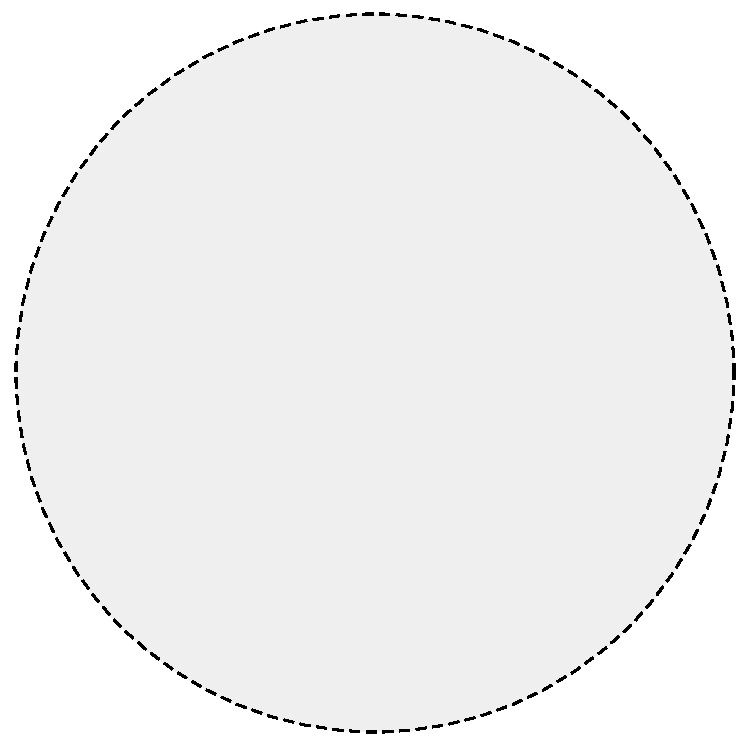
\includegraphics[align=c,width=1.5in]{NotClosedBounded}}\quad
			\fbox{\includegraphics[align=c,width=1.5in]{ClosedBounded}}
		\end{minipage}
		\caption{(Left to Right) 1.~Not Closed + Not Bounded; 2.~Closed + Not Bounded; 3.~Not Closed + Bounded; 4.~Closed + Bounded. Note: The outside boxes are not included in any of the regions.}
	\end{figure}
	
	\newpage
	
	\Q Great! Now, can I maximize/minimize a function subject to $\geq 1$ constraints? If so, how?
	
	\Short You can, using Lagrange Multipliers!
	
	\Long  If you have a two- (or three-)variable function $f(x,y)$ (or $f(x,y,z)$) subject to \textbf{one} constraint $g(x,y)=\text{constant}$ (or $g(x,y,z)=\text{constant}$), then $\nabla f = \lambda\nabla g$ for some real number $\lambda$. Assuming $f$ is two-variable, this yields three equations:
	\begin{enumerate}
		\item $f_x=\lambda g_x$
		\item $f_y=\lambda g_y$
		\item $g(x,y)=\text{constant}$
	\end{enumerate}
	Now: Solve these for points $(x,y)$; evaluate $f(x,y)$ for all those points; and pick out which of the $f(x,y)$-values are largest and smallest. These are the maxes and mins, respectively.
	
	Likewise, if you have a three-variable function $f(x,y,z)$ subject to \textbf{two} constraints $g(x,y,z)=\text{constant}$ and $h(x,y,z)=\text{constant}$, you have $\nabla f = \lambda\nabla g + \mu\nabla h$. Now, this yields \textit{five} equations:
	\begin{enumerate}
		\item $f_x=\lambda g_x + \mu h_x$
		\item $f_y=\lambda g_y + \mu h_y$
		\item $f_z=\lambda g_z + \mu h_z$
		\item $g(x,y,z)=\text{constant}$
		\item $h(x,y,z)=\text{constant}$
	\end{enumerate}
	Now, you do the same as above: Solve these for points $(x,y,z)$; evaluate $f(x,y,z)$ for all those points; and pick out which of the $f(x,y,z)$-values are largest and smallest. These are the maxes and mins, respectively.
	
	\Q How is the Lagrange thing related to the absolute max/min thing above?
	
	\Ans By changing the two-variable constraint $g(x,y)=\text{constant}$ into $g(x,y)\leq\text{constant}$, you may end up with a closed, bounded region in $\Reals^2$.
	
	If so, and if $f(x,y)$ is continuous on the region $g(x,y)\leq\text{constant}$, then we can use the extreme value theorem to know: 
	\begin{enumerate}[label=(\alph*)]
		\item$f$ attains absolute maxes \textit{and} mins on that region; and 
		\item these maxes/mins lie either at critical points of the region or on the region's boundary.
	\end{enumerate}.
	Finally, by noting that the Lagrange multiplier method has already checked the \textbf{boundary} of this region, we only need to compare the $f(x,y)$ values we got above to the values of $f$ at critical points living inside the region to find which are absolute maxes and absolute mins.
\end{document}